% XCircuit output "ri_realim.tex" for LaTeX input from ri_realim.eps
\def\putbox#1#2#3#4{\makebox[0in][l]{\makebox[#1][l]{}\raisebox{\baselineskip}[0in][0in]{\raisebox{#2}[0in][0in]{\scalebox{#3}{#4}}}}}
\def\rightbox#1{\makebox[0in][r]{#1}}
\def\centbox#1{\makebox[0in]{#1}}
\def\topbox#1{\raisebox{-0.60\baselineskip}[0in][0in]{#1}}
\def\midbox#1{\raisebox{-0.20\baselineskip}[0in][0in]{#1}}
   \scalebox{1}{
   \normalsize
   \parbox{7.76042in}{
   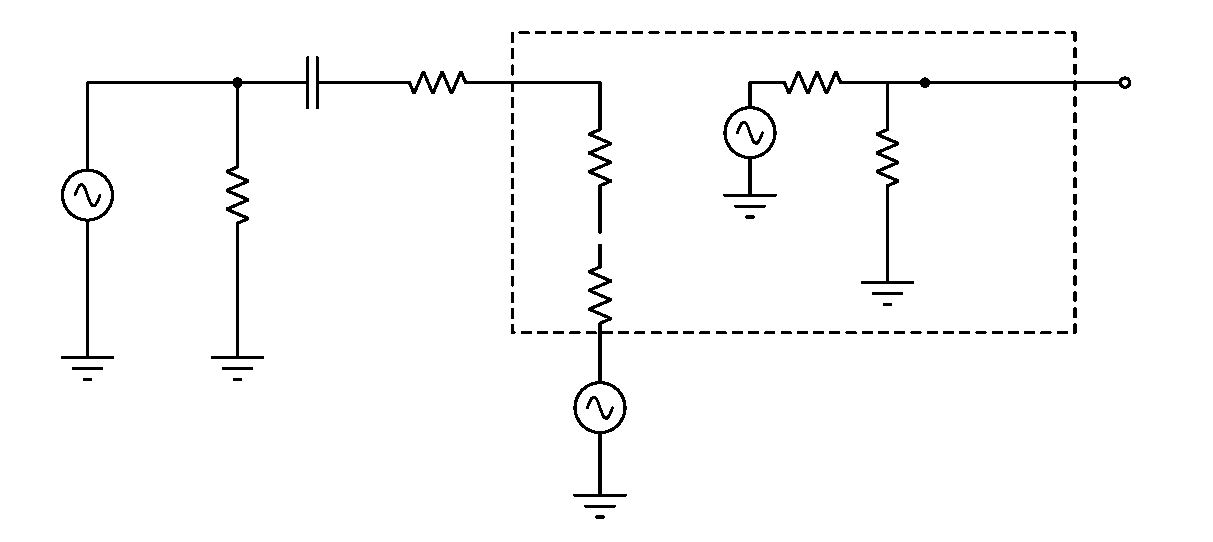
\includegraphics[scale=1]{ri_realim}\\
   % translate x=1008 y=492 scale 0.38
   \putbox{4.06in}{2.45in}{1.20}{R20}%
   \putbox{2.64in}{3.20in}{1.20}{R16}%
   \putbox{1.81in}{3.20in}{1.20}{C1}%
   \putbox{1.64in}{2.12in}{1.20}{R19}%
   \putbox{0.06in}{2.20in}{1.20}{Vi}%
   \putbox{7.56in}{2.87in}{1.20}{Vo}%
   \putbox{5.22in}{2.62in}{1.20}{Ro}%
   \putbox{5.97in}{2.37in}{1.20}{RF1+RF2}%
   \putbox{4.06in}{1.54in}{1.20}{RF//+RF2}%
   \putbox{4.14in}{0.70in}{1.20}{vf}%
   } % close 'parbox'
   } % close 'scalebox'
   \vspace{-\baselineskip} % this is not necessary, but looks better
